\documentclass[10pt,a4paper,UTF8]{article}
\usepackage{zclorg}
\author{emacsun}
\date{}
\title{递归问题:瑞士披萨}
\hypersetup{
 pdfauthor={emacsun},
 pdftitle={递归问题:瑞士披萨},
 pdfkeywords={},
 pdfsubject={本文探讨具体数学第一章递归问题中的第二个问题:瑞士披萨},
 pdfcreator={Emacs 25.0.50.1 (Org mode 8.3.2)}, 
 pdflang={English}}
\begin{document}

\maketitle\xiaosihao
\tableofcontents\newpage\newpage


\section{问题描述}
\label{sec:orgheadline1}


用一把披萨刀直直的切 \(n\)刀,可以最多获得多少块披萨(不要求每块披萨形状一样)。更学术一点的表述为:平面上 \(n\)条直线所能界定的区域的最大个数 \(L_{n}\)是多少?

\section{从小入手}
\label{sec:orgheadline2}

按照我们探讨汉诺塔的思路,先从小入手。

\begin{figure}[htb]
\centering
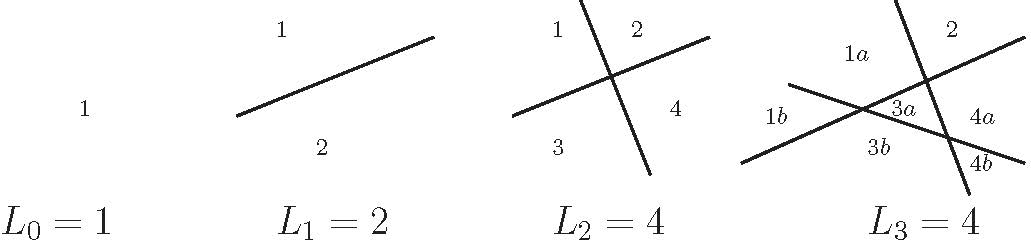
\includegraphics[width=0.5\textwidth]{../../img/pissa.jpg}
\caption{切1,2,3刀的结果}
\end{figure}

可以看出第三条直线对原有的三个区域( 区域1,3,4)进行了分割,使得区域个数增加了三个,而第三条直线与原来的两条直线有交点。推而广之,第 \(n\)条直线可以使得区域个数增加 \(k\)个,当前仅当第 \(n\)条直线对已有的 \(k\)个区域进行了分割;第 \(n\)条直线对已有的 \(k\)个区域进行分割,当前仅当它与已有的 \(k-1\) 条直线有交点。两条直线之多有一个交点,因此这条新的直线与已经存在的 \(n-1\) 条直线至多有 \(n-1\) 个交点,故必有 \(k\le n\)。

\section{披萨递归式}
\label{sec:orgheadline3}

通过上节分析,有:

\begin{equation}
\label{eq:1}
L_{n} \le L_{n-1} + n, n>0
\end{equation}

另外,很容易分析,上式中的等号可以达到。只需要在纺织第 \(n\) 条直线时,使得其不予其他直线中的任何一条平行,且新的直线不经过任何已经存在的交点。于是,披萨递归式演变为:

\begin{equation}
\label{eq:2}
L_{n} = L_{n-1} + n, n>0
\end{equation}

对于该递归式,我们需要一个闭式的解(关于什么样的解才是闭式解,请参考《具体数学》第6页的部分论述,此处省略若干字)。通过把披萨递归式展开,我们发现:

\begin{eqnarray}
\label{eq:3}
L_{n} &=& L_{n-1} +n \\
&=& L_{n-2} + (n-1) + n \\
&=& L_{n-3} + (n-2) + (n-1) + n \\
&\vdots& \vdots \\
&=& L_{0} + 1 + 2 + \ldots + n \\
\end{eqnarray}

显然:

\begin{equation}
\label{eq:4}
L_{n} = 1 + \frac{n(n+1)}{2} ,n > 0
\end{equation}

\section{拓展1:锯齿刀}
\label{sec:orgheadline4}

现在考虑切割披萨问题的一个变形。假设我们用折线代替直线,每一条折现包含一个锯齿,就像等腰三角形去掉底一样。如下图所示,平面上由 \(n\) 条这样的折线所界定的区域数 \(Z_{n}\) 最多是多少?

\begin{figure}[htb]
\centering
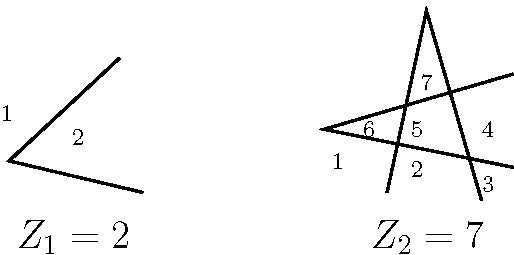
\includegraphics[width=5cm]{../../img/pissaz.jpg}
\caption{折形曲线划分平面}
\end{figure}

从上图的小规模实现可以发现,除了两条直线不经过它们的交点延伸出去外,一条折线和两条直线相同:

\begin{figure}[htb]
\centering
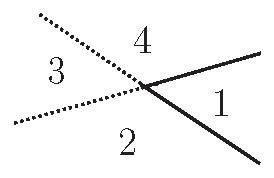
\includegraphics[width=5cm]{../../img/zigzag.jpg}
\caption{一条折线和两条直线}
\end{figure}

区域2,3,4对于两条直线来说是不同的区域,但是在一条折线的情况下是单独的一个区域,于是一条折线相对于两条直线减少了两个区域。如果每条折线的顶点都位于它与其他直线交点之外,每一条折线损失两个区域是固定不变的,于是有:
\begin{equation}
\label{eq:5}
Z_{n} = L_{2n} -2n = \frac{2n(2n+1)}{2} +1 -2n = 2n^{2} -n +1, n\ge 0
\end{equation}

相比较而言,如果 \(n\) 足够大,则 \(L_{n}\)和 \(Z_{n}\) 有如下关系:
\begin{eqnarray}
\label{eq:6}
L_{n} &\sim & \frac{1}{2}n^{2} \\
Z_{n} &\sim & 2n^{2}
\end{eqnarray}

即,有 当 \(n \rightarrow \infty\),\(Z_{n} = 4 L_{n}\)
\section{拓展2:Z形刀}
\label{sec:orgheadline5}


假设有 \(n\) 条Z行曲线所定义的区域最大个数是多少?如图所示。 每条Z行线由两条平行的无线半直线和一条直线段组成。

\begin{figure}[htb]
\centering
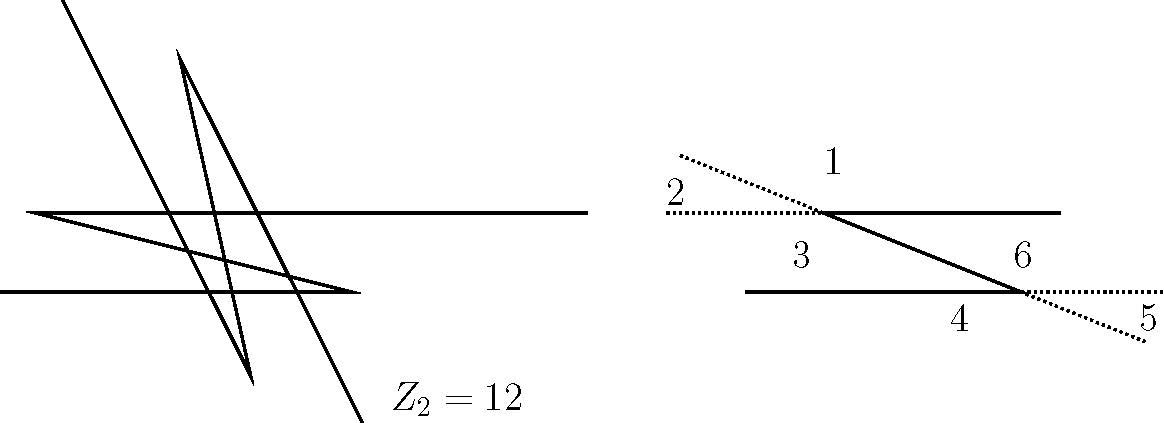
\includegraphics[width=5cm]{../../img/pissazz.jpg}
\caption{一条折线和两条直线}
\end{figure}

如图所示,分析知: 一条Z线划分生成的区域相当于三条曲线,只是Z形曲线划分的区域比三条曲线要少了5个,其中四个区域是因为直线的不完整造成的,一个区域是因为Z型曲线的两条平行线造成的。所以:

\begin{equation*}
Z_{n} = L_{3n} - 5n = \frac{3n(3n+1)}{2} + 1 - 5n =  \frac{9n^{2}}{2} - \frac{7n}{2} +1
\end{equation*}

\section{拓展3: 三维奶酪问题}
\label{sec:orgheadline6}


在一块后奶酪上画出五道直的刀痕,可以得到多少块奶酪?( 在划奶酪时,奶酪必须保持在它原来的位置上,且每道切痕必定与三维空间中的一个平面相对应。) 求 \(P_{n}\) 的一个递归关系,这里 \(P_{n}\) 表示 \(n\) 个不同的平面所能定义的三维区域的最大个数。
\end{document}
